\documentclass{beamer}
\usetheme{default}


\title{Implémentation du protocole CRS d'échange de clefs à base d'isogénies }
\author{Hugo Nartz, Cl\'ement Jacquot}
\date{16 F\'evrier 2022}

\AtBeginSubsection[]
{
  \begin{frame}<beamer>{Outline}
    \tableofcontents[currentsection,currentsubsection]
  \end{frame}
}

\begin{document}

%%%%%%%%%%%%%%%%%%%%%%%%%%%%%%%%%%%%%%%%%%%%%%%%%%%%%%
%% Titlepage
%%%%%%%%%%%%%%%%%%%%%%%%%%%%%%%%%%%%%%%%%%%%%%%%%%%%%%
\begin{frame}
  \titlepage
\begin{figure}[h]
\centering
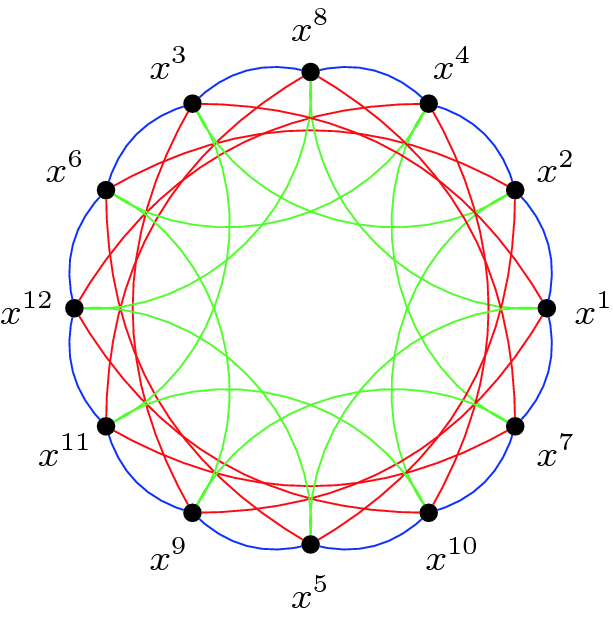
\includegraphics[scale=0.5]{../figs/isoGraph}
\end{figure}
\end{frame}

%%%%%%%%%%%%%%%%%%%%%%%%%%%%%%%%%%%%%%%%%%%%%%%%%%%%%%
%% Toc
%%%%%%%%%%%%%%%%%%%%%%%%%%%%%%%%%%%%%%%%%%%%%%%%%%%%%%
\begin{frame}{}
  \tableofcontents
\end{frame}

\section{Le protocol CRS}
%%%%%%%%%%%%%%%%%%%%%%%%%%%%%%%%%%%%%%%%%%%%%%%%%%%%%%
%% Isogeny graphs
%%%%%%%%%%%%%%%%%%%%%%%%%%%%%%%%%%%%%%%%%%%%%%%%%%%%%%
\begin{frame}{Courbes elliptiques et isog\'enies}
	\begin{thm}
		efe
	\end{thm}
\end{frame}

\begin{frame}{Réduite et quotients}
\begin{itemize}
    \item{}
\end{itemize}
\end{frame}

\begin{frame}{Proposition}
\begin{itemize}
    \item{Il existe deux suites $(P_n)$ et $(Q_n)$ de polynomes tels que:}
    \item{$P_n$ et $Q_n$ ne dépendent que de $X_0,\cdots,X_n$}
    \item{$P_0 = X_0, P_1 = X_0 X_1+1$ et $Q_0 = 1, Q_1 = X_1$}
    \item{$\forall n \geq 2: P_n = X_nP_{n-1}+P_{n-2}$ et $Q_n = X_n Q_{n-1}+Q_{n-2}$}
    %deg ?
\end{itemize}
\end{frame}

\begin{frame}{Théorème}
\begin{itemize}
    \item{$\forall n \geq 0$}
    \item{$F_n = [X_0,\cdots, X_n] = \frac{P_n}{Q_n}$}
\end{itemize}
\end{frame}

\section{Algorithme des fractions continues}
\begin{frame}{Algorithme}
\begin{itemize}
    \item{$\theta \in \mathbb{R}$}
    \item{$a_0 = [\theta]$}
    \item{Si $\theta\in \mathbb{Z}$ alors $\theta = a_0$ fin}
    \item{Sinon $\theta-a_0 \in ]0,1[$ et il existe $\theta_1$ tel que $\theta = a_0 + \frac{1}{\theta_1}$, on réitère le processur pour $\theta = \theta_1$ et $a_1=[\theta_1]$}
    \item{L'algorithme termine si et seulement si il existe $n$ tel que $\theta_n = [a_n]$}
\end{itemize}
\end{frame}




\end{document}
